\documentclass[aspectratio=169,11pt]{beamer}
\mode<presentation> {
\usetheme{Madrid}
% \usecolortheme{albatross}
}

\usepackage[brazil]{babel}
\usepackage[utf8]{inputenc}
\usepackage{graphicx} 
\usepackage{booktabs} 



\institute[UEA] 
{
%================= logos no meio =====================
\vspace*{-0.35cm}

\includegraphics[width=1.8cm]{img/logo-uea.png}
\hspace*{0.25cm}~%

\includegraphics[width=1.8cm]{img/logo-neo.png}
\vspace*{0.35cm}\\
Núcleo de Engenharia e Otimização -- NEO \\
Escola Superior de Tecnologia -- EST\\
Universidade do Estado do Amazonas -- UEA\\
%\medskip
%\texttt{\{lods.eng,ronety\}@uea.edu.br} % emails
}
\date{\today}

\AtBeginSection[]
{
\begin{frame}
\frametitle{Conteúdo}
\tableofcontents[currentsection]
\end{frame}
}

%%%%%%%% title %%%%%%%%
\title[Interim Report]{Experimental Cloud using Commodity Hardware} 

%%%%%%%% Author %%%%%%%%
\author[111601008]{Kaushal Kishore, Sandeep Chandran} 

\begin{document}
\begin{frame}
\titlepage 

\end{frame}

\begin{frame}
\frametitle{Conteúdo} 
\tableofcontents 
\end{frame}

%%%%%%%% slides %%%%%%%%
\section{Introduction} 
\begin{frame}{Cloud}
    Essentially, it is a term used to describe a global network of servers, which are hooked together and meant to operate as a single ecosystem.
    \begin{center}
        
\includegraphics[width=0.5\textwidth]{img/cloud-computing.png}
    \end{center}
\end{frame}

\begin{frame}{Cloud Services}
    \begin{center}
        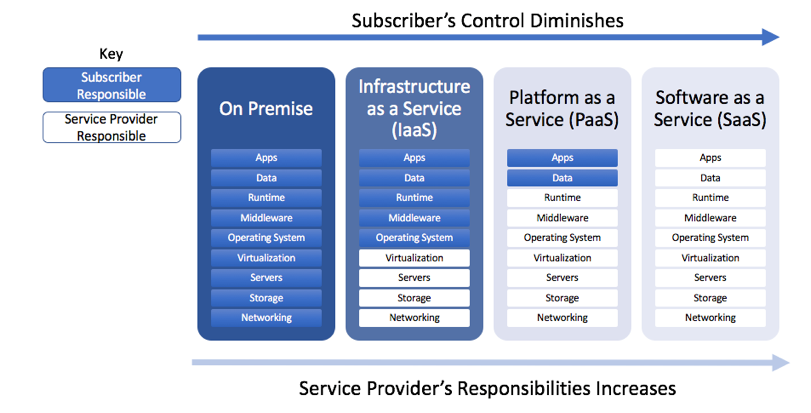
\includegraphics{img/cloud-services-model.png}
    \end{center}
\end{frame}

\begin{frame}{Pros \& Cons}
    \begin{block}{Pros}
        \begin{itemize}
            \item Reduced hardware equipment for end-users
            \item Improved performance
            \item Lower H/W and S/W maintainence
            \item Instant software updates
            \item Improved disaster recovery
            \item Less expensive
            \item Accessibility
        \end{itemize}
    \end{block}

    \begin{block}{Cons}
        \begin{itemize}
            \item Requires good internet connection \& bandwidth
            \item Limited control on infrastructure
        \end{itemize}
    \end{block}
\end{frame}

\begin{frame}{Problem Statement}
    \begin{block}{Experimental Cloud using Commodity Hardware}
        The objective of this project is to create an experimental cloud by repurposing commodity hardware. The cloud we create would be made available to students as virtual desktops which may be used to host web services which can vary from simple static page to complex web applications.
    \end{block}
\end{frame}

\section{MaaS}
\begin{frame}{Metal-as-a-Service: MaaS}
    \begin{block}{Bare metal cloud}
        Bare metal cloud is an environment in which physical, dedicated servers can be provisioned to customers with cloud-like ease and speed. \linebreak
        \linebreak
        Bare metal cloud customers are given access to the entire processing power of individual servers, as well as any storage, networking or other services they require.
    \end{block}
\end{frame}

% \begin{frame}{IaaS vs. MaaS}

%     \begin{center}
%         Is there any difference between IaaS \& MaaS?
%     \end{center}

% \end{frame}

% \begin{frame}{IaaS vs. MaaS}

%     \begin{center}
%         This depends on the view point.
%     \end{center}

% \end{frame}

% \begin{frame}{IaaS vs. MaaS}

%     \begin{center}
%         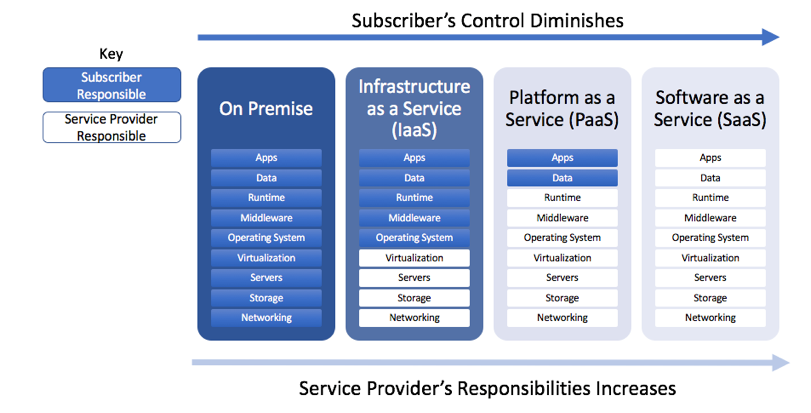
\includegraphics{img/cloud-services-model.png}
%     \end{center}

% \end{frame}

% \begin{frame}{IaaS vs. MaaS}

%     Many define IaaS as the provision of virtual resources only. Some include dedicated servers in their definition.\\

%     \vspace*{0.35cm}

%     On a virtual IaaS, one has no knowledge of or control over the actual infrastructure on which your services are built. The provider has control of these and your services are abstracted from them.\\

%     \vspace*{0.35cm}

%     With bare metal you get control of the full stack, from the tin right up to the user interface, and can optimise utilisation and performance to a granular level, something you simple cannot do in a virtualised environment.

% \end{frame}

\section{Progress Report}
\begin{frame}{Progress Report}
    \begin{block}{MAAS in VENV}
        The problem statement is to repurpose the commodity hardware to create an experimental cloud. 
        \linebreak
        \linebreak
        At present we don't have access to those hardwares hence we are conducting our experiments in virtual environment.
    \end{block}
\end{frame}

\begin{frame}{Progress Report}
    \begin{block}{MAAS in VENV}
        Successfully deployed a MAAS based cloud in virtual environment.
    \end{block}
\end{frame}

\section{Conclusion}
\begin{frame}{Conclusion}
    \begin{block}{Future Work}
        \begin{itemize}
            \item Moving to physical hardwares.
        \end{itemize}
    \end{block}
\end{frame}

% \section{}
% \begin{frame}{Justificativa: blocos}
\begin{block}{Block 1}
Lorem ipsum dolor sit amet, consectetur adipiscing elit. Integer lectus nisl, ultricies in feugiat rutrum, porttitor sit amet augue. Aliquam ut tortor mauris. Sed volutpat ante purus, quis accumsan dolor.
\end{block}

\begin{block}{Block 2}
Pellentesque sed tellus purus. Class aptent taciti sociosqu ad litora torquent per conubia nostra, per inceptos himenaeos. Vestibulum quis magna at risus dictum tempor eu vitae velit.
\end{block}

\end{frame}

% \section{Objetivos}
% \begin{frame}{Objetivos}
\begin{block}{Objetivo Geral}
O objetivo geral é fazer um algoritmo para calcular expressão gênica a partir de uma parte da sequência de RNA
\end{block}

\begin{block}{Objetivos Específicos}
\begin{itemize}
    \item Objetivo específico 1
    \item Objetivo específico 2
    \item Objetivo específico 3
    \item Objetivo específico 4
\end{itemize}
\end{block}

    
\end{frame}

% \section{Fundamentação Teórica}
% \begin{frame}{Fundamentação Teórica}
\begin{itemize}
    \item Nós utilizamos essa abordagem
    \item Assim assim
    \item Assado
\end{itemize}
    
\end{frame}

\begin{frame}{Fundamentação Teórica}
Nesta \textbf{abordagem} nós fizemos bla bla bla
\medskip

\begin{itemize}
    \item Exemplo de item
    \medskip
    \item Exemplo de item
\end{itemize}    
\medskip

\begin{theorem}[Mass--energy equivalence]
$E = mc^2$
\end{theorem}

\end{frame}

% \section{Metodologia}
% \begin{frame}{Metodologia}
\begin{columns}[c] % The "c" option specifies centered vertical alignment while the "t" option is used for top vertical alignment

\column{.45\textwidth} % Left column and width
\textbf{Passos da metodologia}
\begin{enumerate}
\item Statement
\item Explanation
\item Example
\end{enumerate}

\column{.5\textwidth} % Right column and width
Explicando alguma coisa ... lorem ipsum dolor sit amet, consectetur adipiscing elit. Integer lectus nisl, ultricies in feugiat rutrum, porttitor sit amet augue. Aliquam ut tortor mauris. Sed volutpat ante purus, quis accumsan dolor.

\end{columns}
\end{frame}

% \section{Resultados}
% \begin{frame}{Resultados}
\begin{table}
\begin{tabular}{l l l}
\toprule
\textbf{Treatments} & \textbf{Response 1} & \textbf{Response 2}\\
\midrule
Treatment 1 & 0.0003262 & 0.562 \\
Treatment 2 & 0.0015681 & 0.910 \\
Treatment 3 & 0.0009271 & 0.296 \\
\bottomrule
\end{tabular}
\caption{Table caption}
\end{table}
\end{frame}

\begin{frame}{Resultados}
    
\begin{figure}
    \centering
    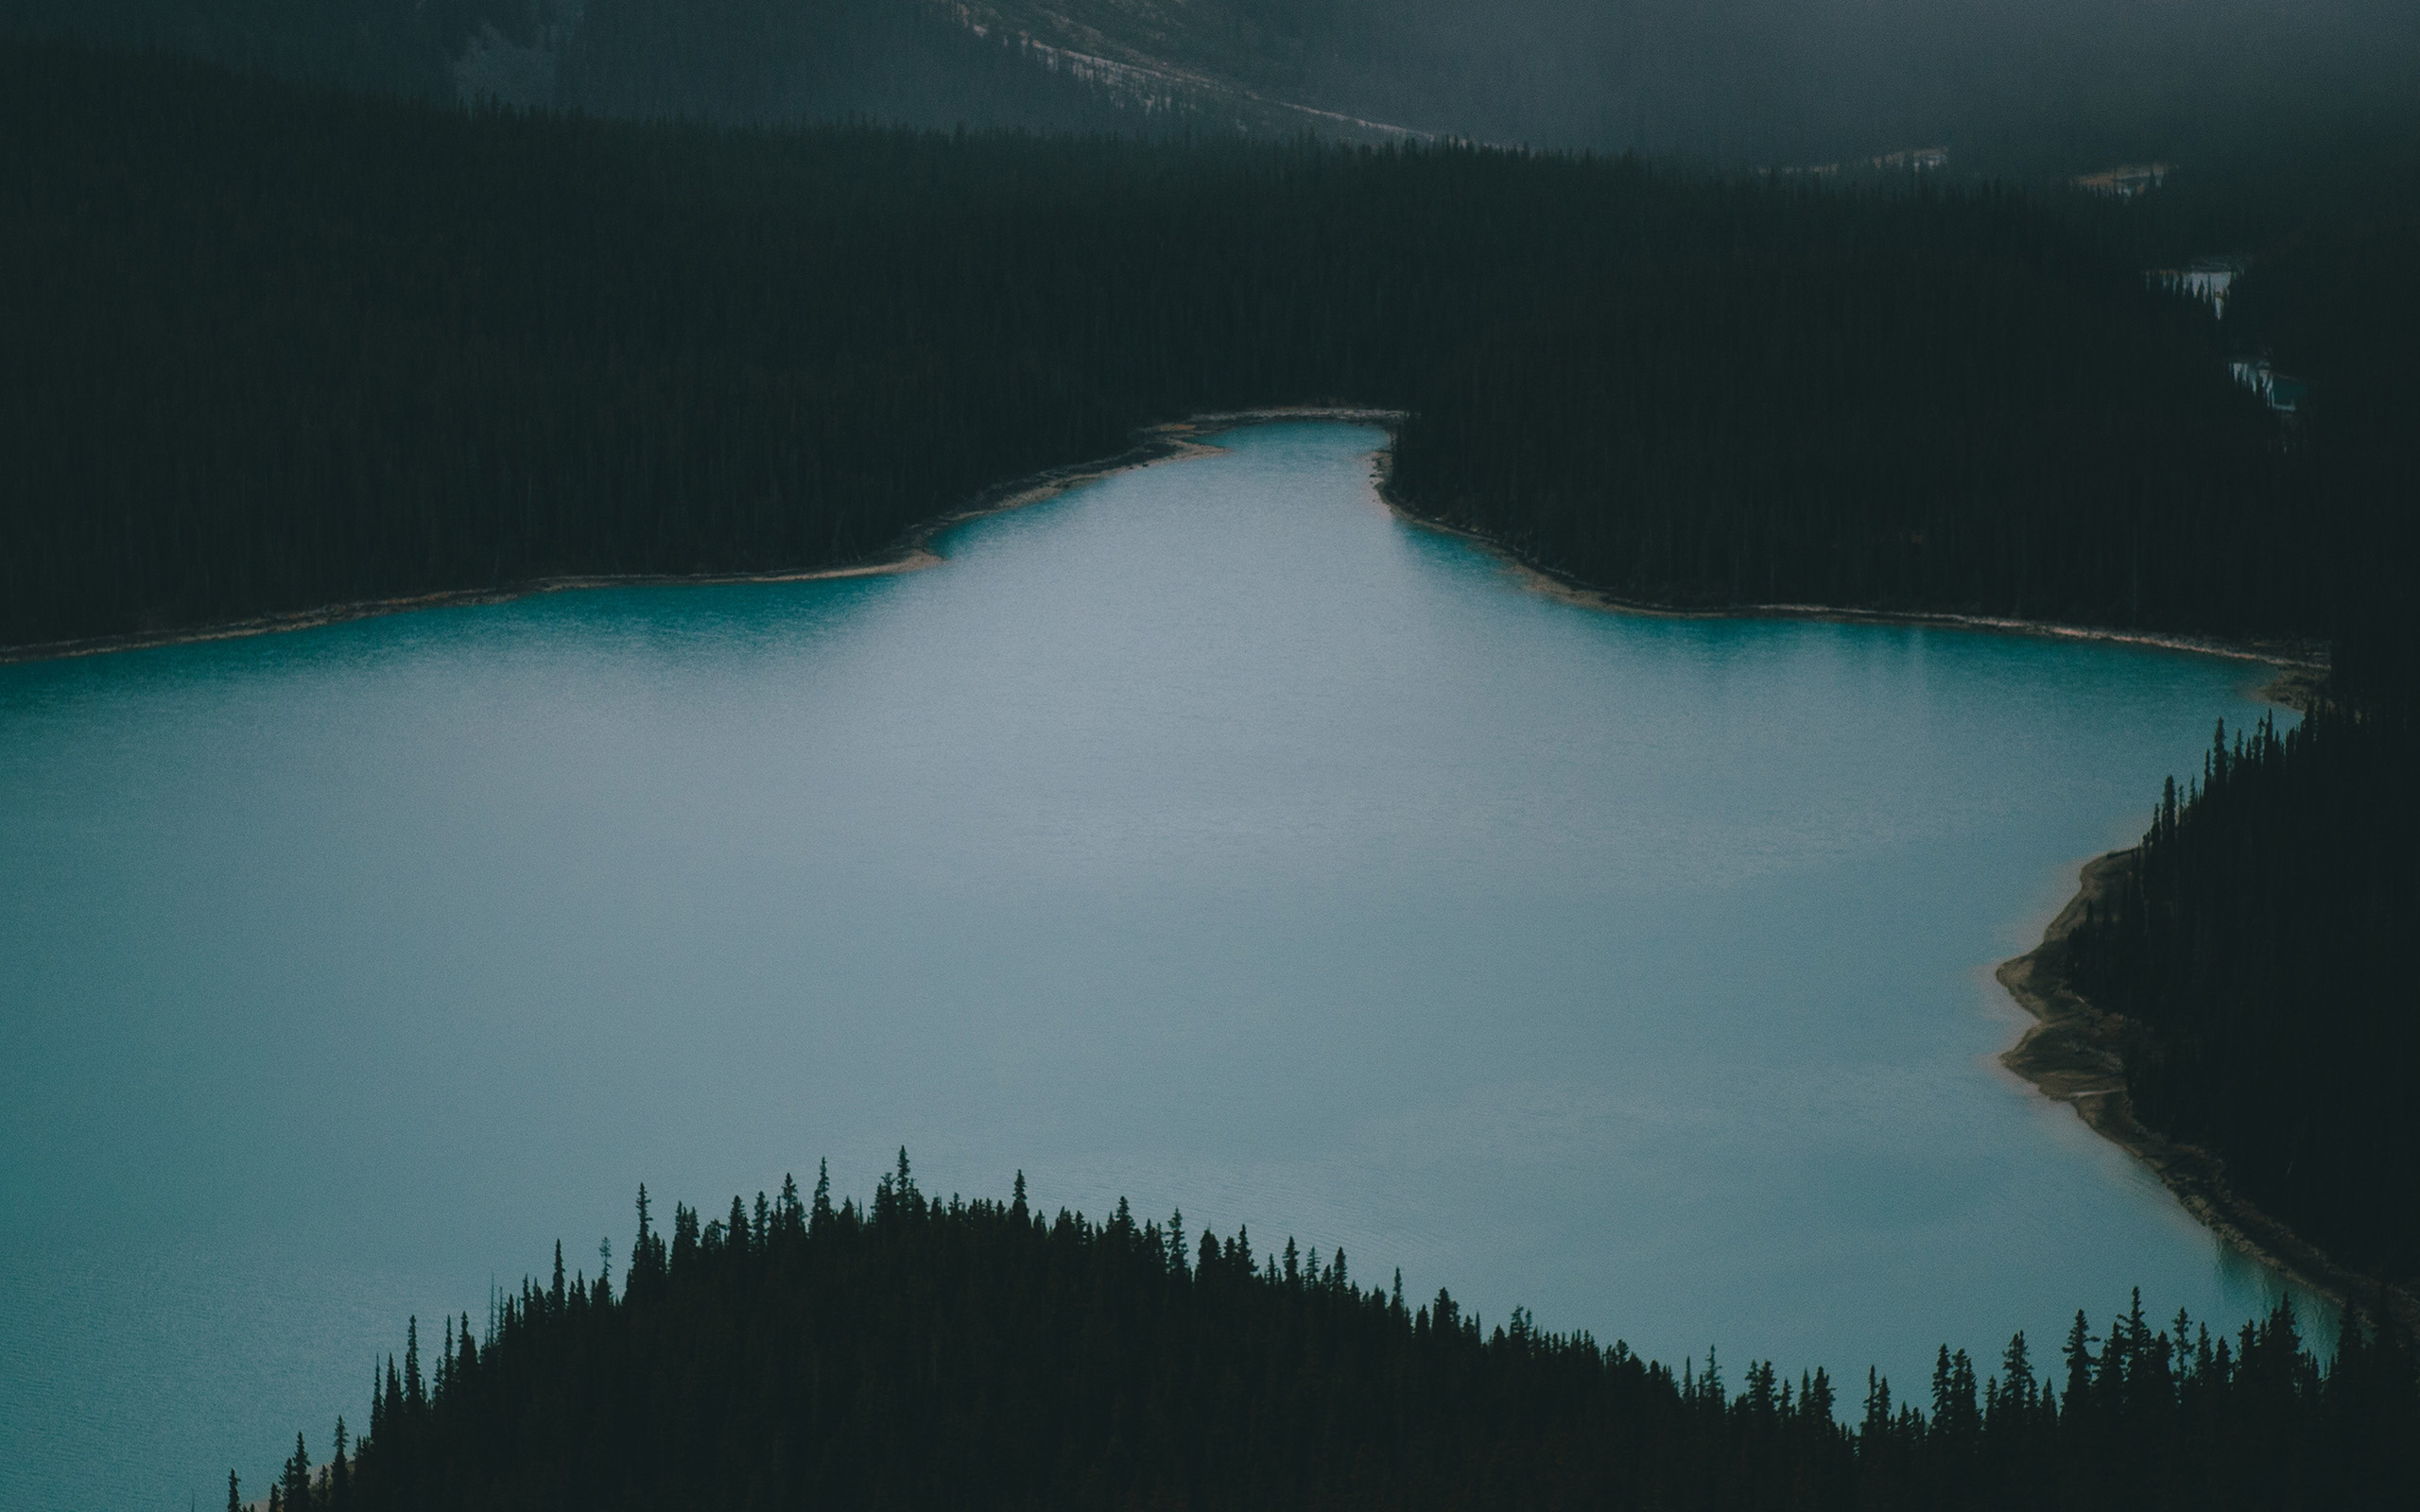
\includegraphics[width=.7\textwidth]{img/river.jpg}
    \caption{Aqui temos a imagem de um lago}
    % \label{fig:my_label}
\end{figure}

\end{frame}

% \section{Conclusão}
% \begin{frame}{Conclusão}
\begin{itemize}
\item more work
\medskip
\item more responsibility
\medskip
\item more satisfaction
\end{itemize}
    
\end{frame}


%%%%%%%% agradecimentos %%%%%%%%
% \begin{frame}{Agradecimentos}
%     \large{Agradeço a fulano, ciclano e beltrano que apoiaram o desenvolvimento dessa pesquisa.}
% \end{frame}
%------------------------------------------------


%------------------------------------------------
%------------------------------------------------
%%%%%%%% referencias %%%%%%%%
% \nocite{*}
% \begin{frame}[allowframebreaks]{Referências}
% \bibliographystyle{unsrt}
% \bibliography{ref.bib}
% \end{frame}


%%%%%%%% repete primeiro slide %%%%%%%%
\begin{frame}
\titlepage 
\end{frame}


\end{document}